\documentclass[]{article}
\usepackage[UTF8]{ctex}
\usepackage{CJK}
\usepackage{lmodern}
\usepackage{amssymb,amsmath}
\usepackage{ifxetex,ifluatex}
\usepackage{fixltx2e} % provides \textsubscript
\ifnum 0\ifxetex 1\fi\ifluatex 1\fi=0 % if pdftex
  \usepackage[T1]{fontenc}
  \usepackage[utf8]{inputenc}
\else % if luatex or xelatex
  \ifxetex
    \usepackage{mathspec}
  \else
    \usepackage{fontspec}
  \fi
  \defaultfontfeatures{Ligatures=TeX,Scale=MatchLowercase}
\fi
% use upquote if available, for straight quotes in verbatim environments
\IfFileExists{upquote.sty}{\usepackage{upquote}}{}
% use microtype if available
\IfFileExists{microtype.sty}{%
\usepackage[]{microtype}
\UseMicrotypeSet[protrusion]{basicmath} % disable protrusion for tt fonts
}{}
\PassOptionsToPackage{hyphens}{url} % url is loaded by hyperref
\usepackage[unicode=true]{hyperref}
\hypersetup{
            pdfborder={0 0 0},
            breaklinks=true}
\urlstyle{same}  % don't use monospace font for urls
\usepackage{color}
\usepackage{fancyvrb}
\newcommand{\VerbBar}{|}
\newcommand{\VERB}{\Verb[commandchars=\\\{\}]}
\DefineVerbatimEnvironment{Highlighting}{Verbatim}{commandchars=\\\{\}}
% Add ',fontsize=\small' for more characters per line
\newenvironment{Shaded}{}{}
\newcommand{\KeywordTok}[1]{\textcolor[rgb]{0.00,0.44,0.13}{\textbf{#1}}}
\newcommand{\DataTypeTok}[1]{\textcolor[rgb]{0.56,0.13,0.00}{#1}}
\newcommand{\DecValTok}[1]{\textcolor[rgb]{0.25,0.63,0.44}{#1}}
\newcommand{\BaseNTok}[1]{\textcolor[rgb]{0.25,0.63,0.44}{#1}}
\newcommand{\FloatTok}[1]{\textcolor[rgb]{0.25,0.63,0.44}{#1}}
\newcommand{\ConstantTok}[1]{\textcolor[rgb]{0.53,0.00,0.00}{#1}}
\newcommand{\CharTok}[1]{\textcolor[rgb]{0.25,0.44,0.63}{#1}}
\newcommand{\SpecialCharTok}[1]{\textcolor[rgb]{0.25,0.44,0.63}{#1}}
\newcommand{\StringTok}[1]{\textcolor[rgb]{0.25,0.44,0.63}{#1}}
\newcommand{\VerbatimStringTok}[1]{\textcolor[rgb]{0.25,0.44,0.63}{#1}}
\newcommand{\SpecialStringTok}[1]{\textcolor[rgb]{0.73,0.40,0.53}{#1}}
\newcommand{\ImportTok}[1]{#1}
\newcommand{\CommentTok}[1]{\textcolor[rgb]{0.38,0.63,0.69}{\textit{#1}}}
\newcommand{\DocumentationTok}[1]{\textcolor[rgb]{0.73,0.13,0.13}{\textit{#1}}}
\newcommand{\AnnotationTok}[1]{\textcolor[rgb]{0.38,0.63,0.69}{\textbf{\textit{#1}}}}
\newcommand{\CommentVarTok}[1]{\textcolor[rgb]{0.38,0.63,0.69}{\textbf{\textit{#1}}}}
\newcommand{\OtherTok}[1]{\textcolor[rgb]{0.00,0.44,0.13}{#1}}
\newcommand{\FunctionTok}[1]{\textcolor[rgb]{0.02,0.16,0.49}{#1}}
\newcommand{\VariableTok}[1]{\textcolor[rgb]{0.10,0.09,0.49}{#1}}
\newcommand{\ControlFlowTok}[1]{\textcolor[rgb]{0.00,0.44,0.13}{\textbf{#1}}}
\newcommand{\OperatorTok}[1]{\textcolor[rgb]{0.40,0.40,0.40}{#1}}
\newcommand{\BuiltInTok}[1]{#1}
\newcommand{\ExtensionTok}[1]{#1}
\newcommand{\PreprocessorTok}[1]{\textcolor[rgb]{0.74,0.48,0.00}{#1}}
\newcommand{\AttributeTok}[1]{\textcolor[rgb]{0.49,0.56,0.16}{#1}}
\newcommand{\RegionMarkerTok}[1]{#1}
\newcommand{\InformationTok}[1]{\textcolor[rgb]{0.38,0.63,0.69}{\textbf{\textit{#1}}}}
\newcommand{\WarningTok}[1]{\textcolor[rgb]{0.38,0.63,0.69}{\textbf{\textit{#1}}}}
\newcommand{\AlertTok}[1]{\textcolor[rgb]{1.00,0.00,0.00}{\textbf{#1}}}
\newcommand{\ErrorTok}[1]{\textcolor[rgb]{1.00,0.00,0.00}{\textbf{#1}}}
\newcommand{\NormalTok}[1]{#1}
\usepackage{longtable,booktabs}
% Fix footnotes in tables (requires footnote package)
\IfFileExists{footnote.sty}{\usepackage{footnote}\makesavenoteenv{long table}}{}
\usepackage{graphicx,grffile}
\makeatletter
\def\maxwidth{\ifdim\Gin@nat@width>\linewidth\linewidth\else\Gin@nat@width\fi}
\def\maxheight{\ifdim\Gin@nat@height>\textheight\textheight\else\Gin@nat@height\fi}
\makeatother
% Scale images if necessary, so that they will not overflow the page
% margins by default, and it is still possible to overwrite the defaults
% using explicit options in \includegraphics[width, height, ...]{}
\setkeys{Gin}{width=\maxwidth,height=\maxheight,keepaspectratio}
\IfFileExists{parskip.sty}{%
\usepackage{parskip}
}{% else
\setlength{\parindent}{0pt}
\setlength{\parskip}{6pt plus 2pt minus 1pt}
}
\setlength{\emergencystretch}{3em}  % prevent overfull lines
\providecommand{\tightlist}{%
  \setlength{\itemsep}{0pt}\setlength{\parskip}{0pt}}
\setcounter{secnumdepth}{0}
% Redefines (sub)paragraphs to behave more like sections
\ifx\paragraph\undefined\else
\let\oldparagraph\paragraph
\renewcommand{\paragraph}[1]{\oldparagraph{#1}\mbox{}}
\fi
\ifx\subparagraph\undefined\else
\let\oldsubparagraph\subparagraph
\renewcommand{\subparagraph}[1]{\oldsubparagraph{#1}\mbox{}}
\fi

% set default figure placement to htbp
\makeatletter
\def\fps@figure{htbp}
\makeatother


\date{}

\begin{document}

\subsection{张晋第十二次作业15091060}\label{header-n0}

\subsection{5.9}\label{header-n3}

\subsubsection{最速下降法}\label{header-n4}

\(\gamma\)=0.9,\(\rho\)=0.01

\paragraph{初始点:(1.2,1.2)}\label{header-n7}

%\begin{figure}
%\centering
%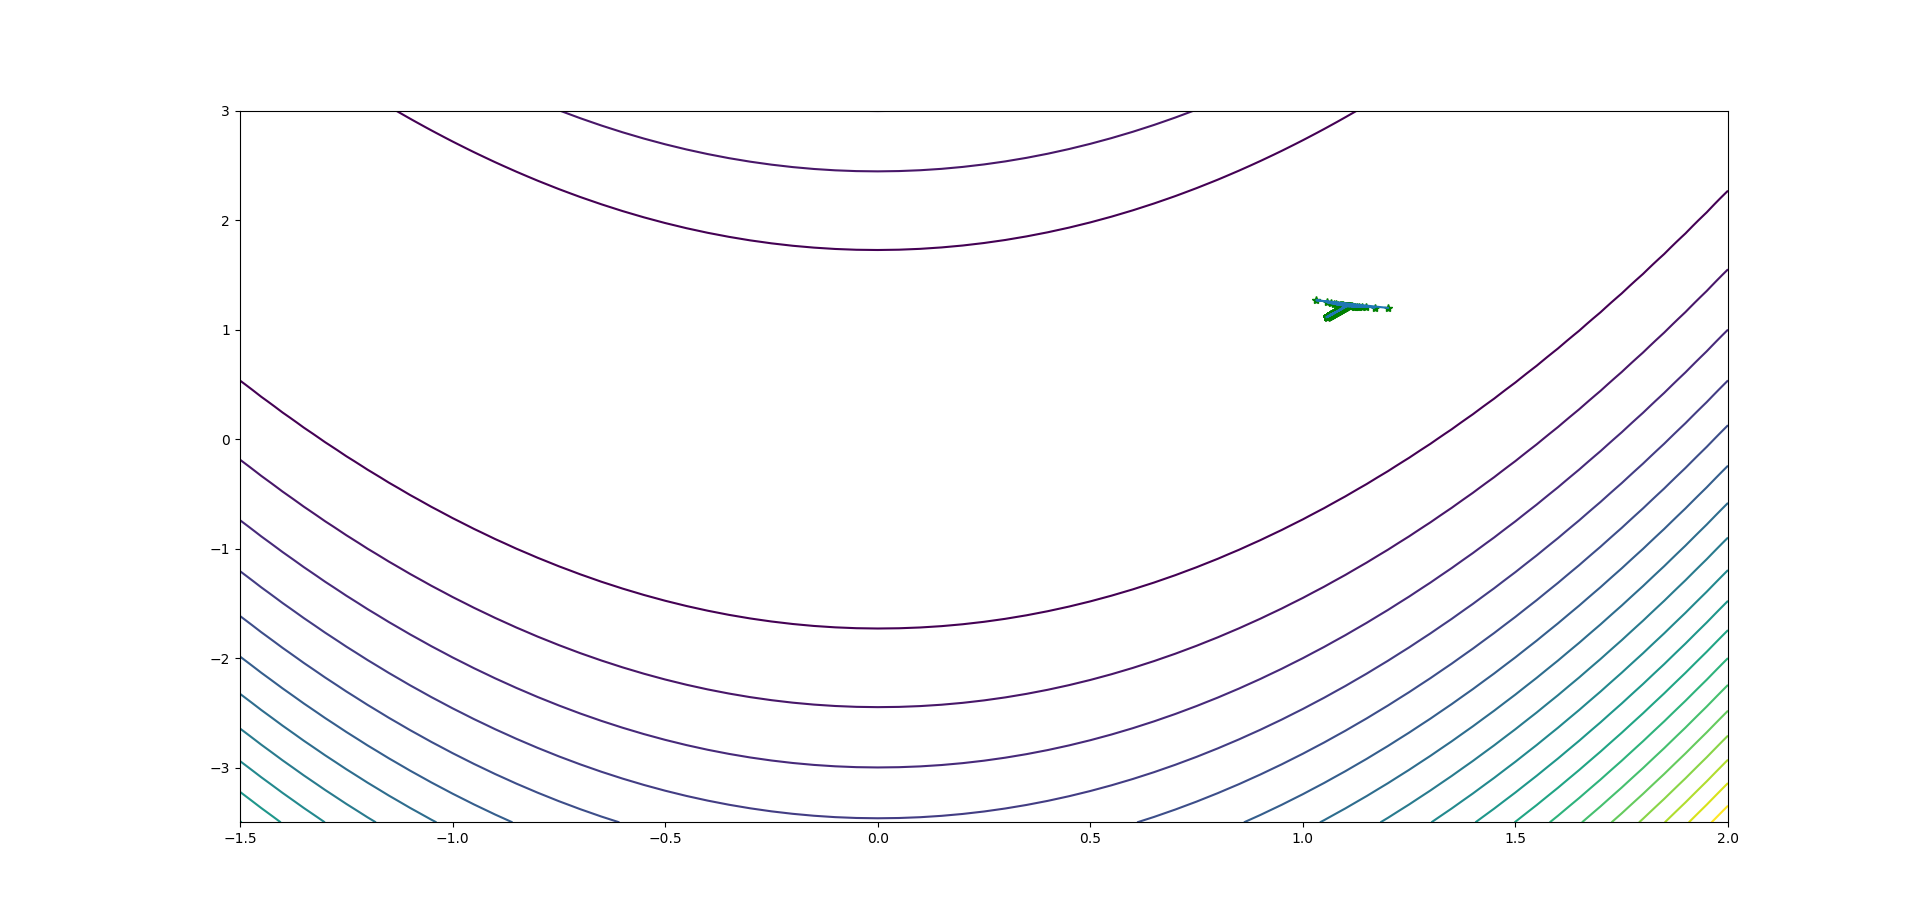
\includegraphics{C:/Users/80693/Desktop/Figure_1-2.png}
%\caption{}
%\end{figure}

第 995 次迭代结果: {[} 1.05604686 1.11578718{]} 步长为: 0.00179701029991
第 996 次迭代结果: {[} 1.05626461 1.11558871{]} 步长为: 0.00179701029991
第 997 次迭代结果: {[} 1.05598175 1.11562688{]} 步长为: 0.00199667811102
第 998 次迭代结果: {[} 1.0562047 1.11541547{]} 步长为: 0.00179701029991
第 999 次迭代结果: {[} 1.05588661 1.11547042{]}

从图像可以看出,结果在最优解左右震荡,尽管接近最优解,但仍然未能很好收敛

\paragraph{初始点:(-1.2,1)}\label{header-n35}

%\begin{figure}
%\centering
%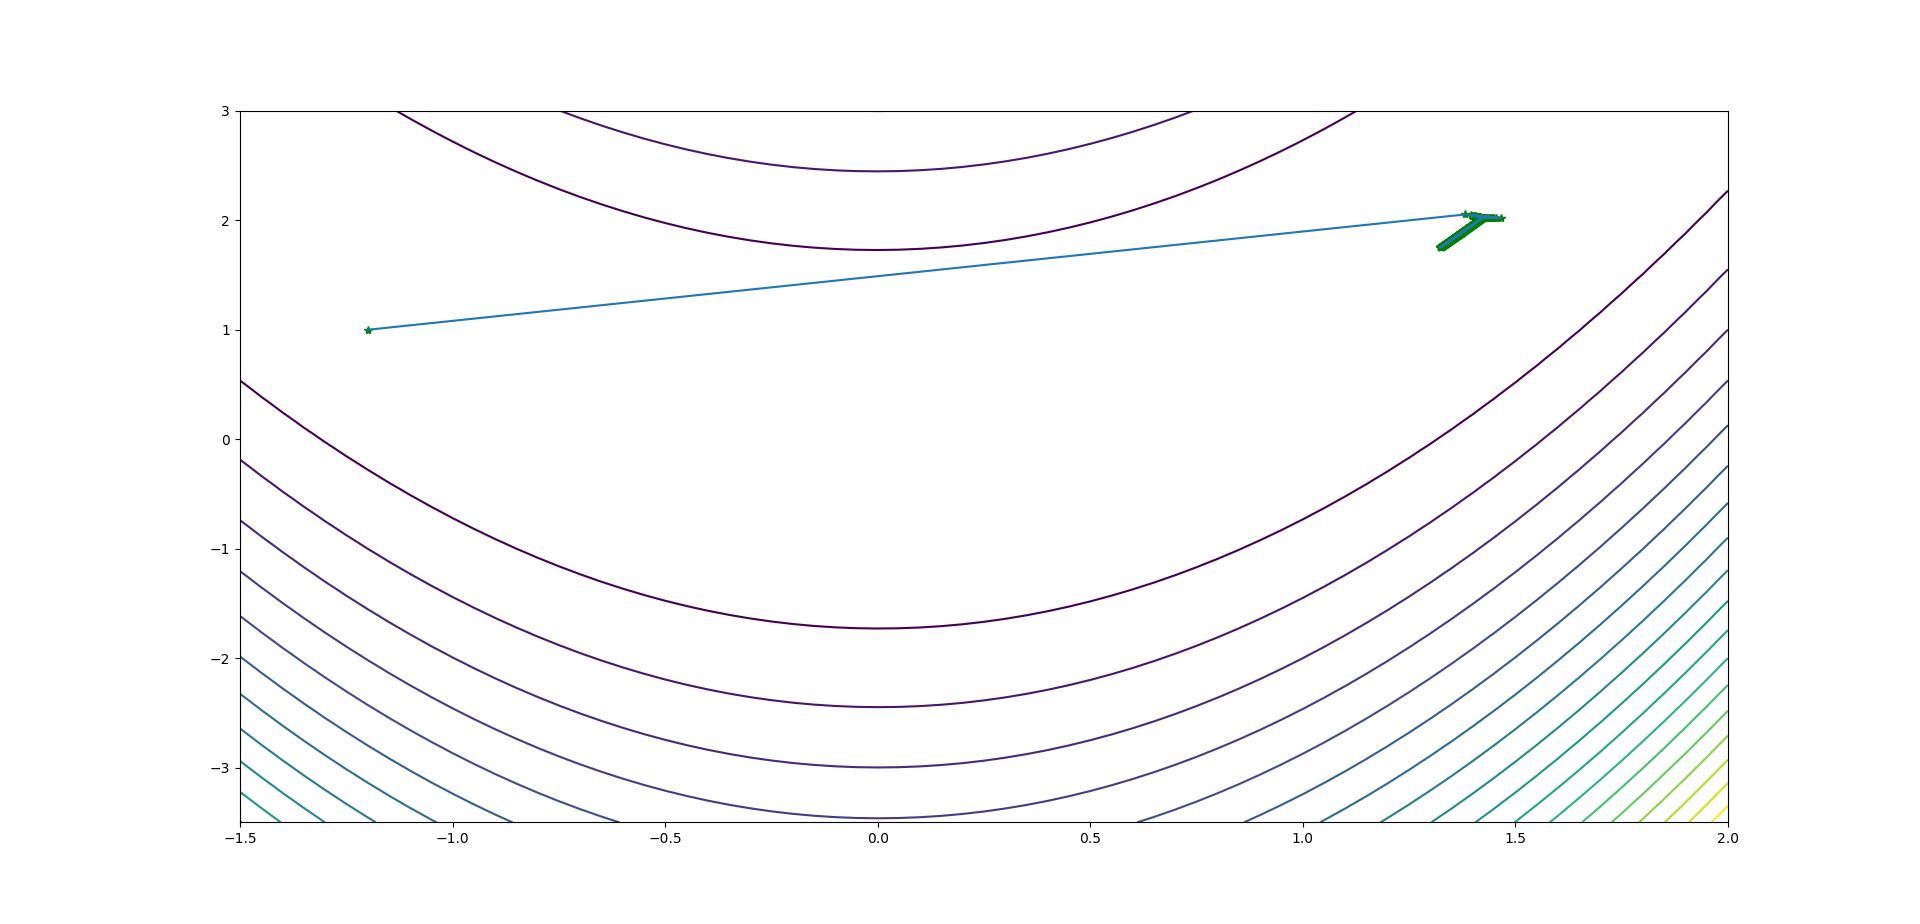
\includegraphics{C:/Users/80693/Desktop/Figure_1-1.png}
%\caption{}
%\end{figure}

第 995 次迭代结果: {[} 1.32340857 1.75425742{]} 步长为: 0.00117901845777
第 996 次迭代结果: {[} 1.32442297 1.75358604{]} 步长为: 0.00131002050864
第 997 次迭代结果: {[} 1.32321891 1.75371971{]} 步长为: 0.00117901845777
第 998 次迭代结果: {[} 1.32421119 1.75305677{]} 步长为: 0.00131002050864
第 999 次迭代结果: {[} 1.32302971 1.75318213{]}

迭代点初始运动得很快,但也和之前一样在最优解附近震荡,收敛很慢

\subsubsection{牛顿法}\label{header-n65}

\(\gamma\)=0.9,\(\rho\)=0.01

\paragraph{初始点:(1.2,1.2)}\label{header-n68}

%\begin{figure}
%\centering
%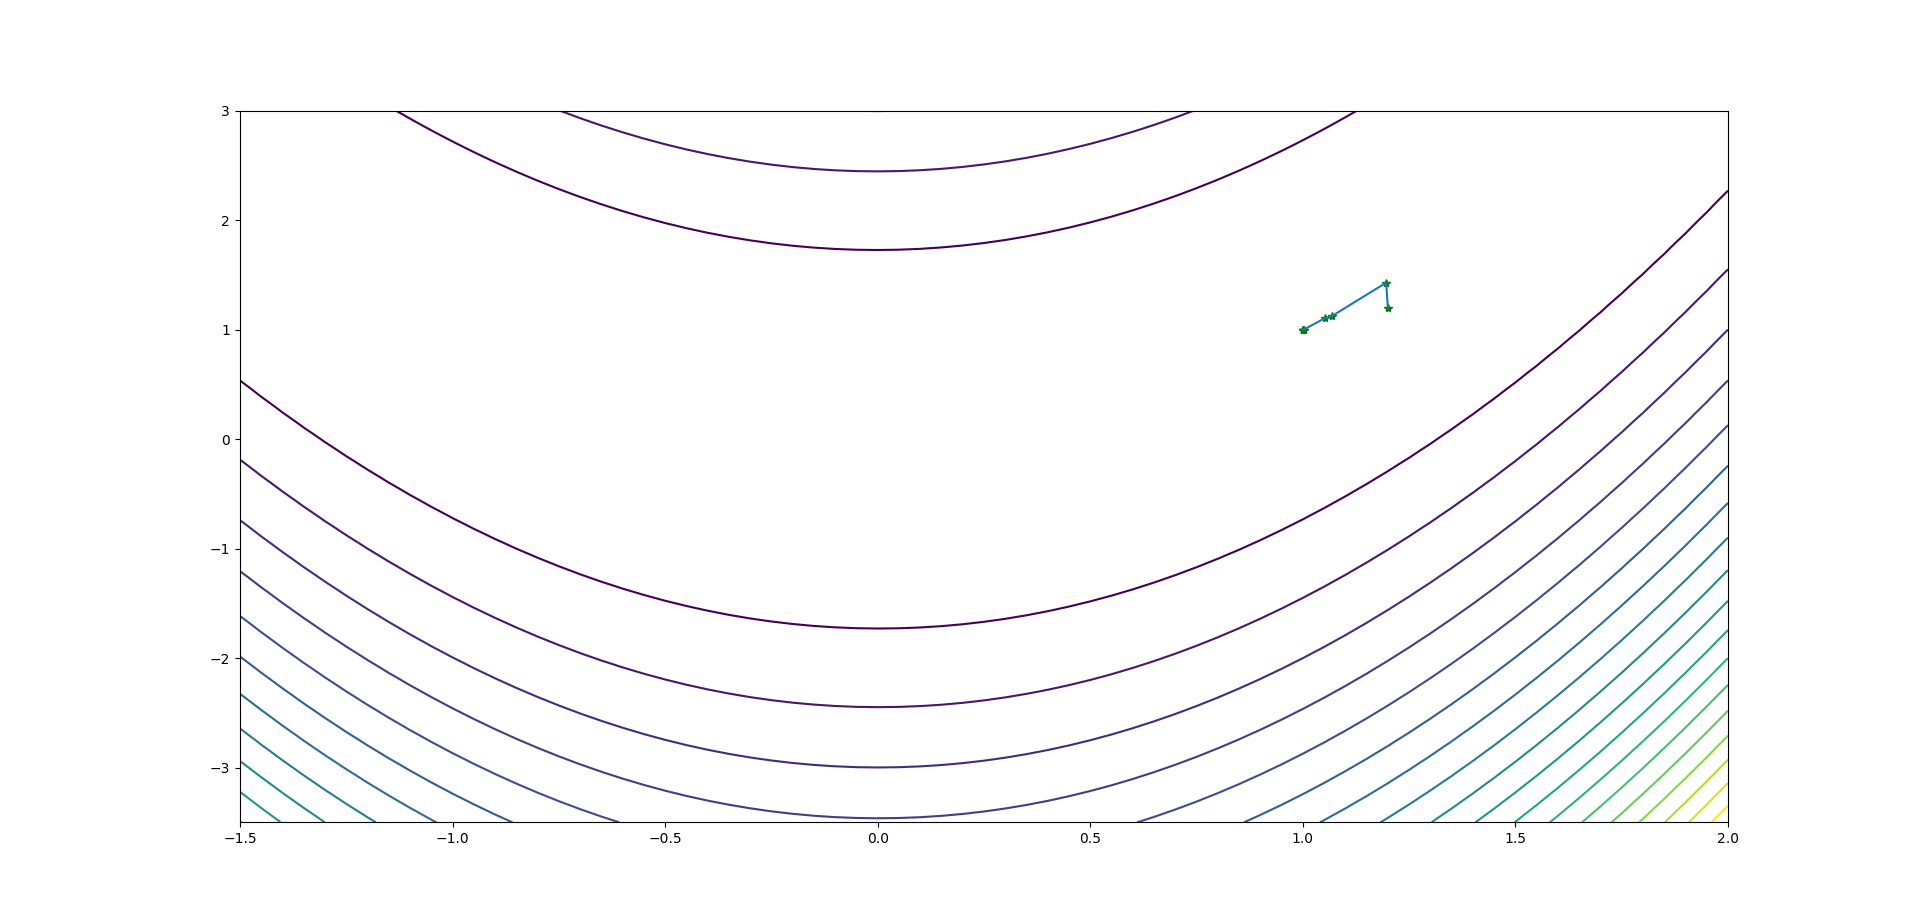
\includegraphics{C:/Users/80693/Desktop/Figure_1-3.png}
%\caption{}
%\end{figure}

第 1 次迭代结果: {[} 1.19591837 1.43020408{]} 步长为: 0.6561 第 2
次迭代结果: {[} 1.0678032 1.12378445{]} 步长为: 1 第 3 次迭代结果: {[}
1.05197555 1.10640204{]} 步长为: 1 第 4 次迭代结果: {[} 1.00247988
1.00251608{]} 步长为: 1 第 5 次迭代结果: {[} 1.00081549 1.00162887{]}
步长为: 1 第 6 次迭代结果: {[} 1.00000045 1.00000024{]} 步长为: 1 第 7
次迭代结果: {[} 1. 1.{]}

\paragraph{初始点:(-1.2,1)}\label{header-n100}

%\begin{figure}
%\centering
%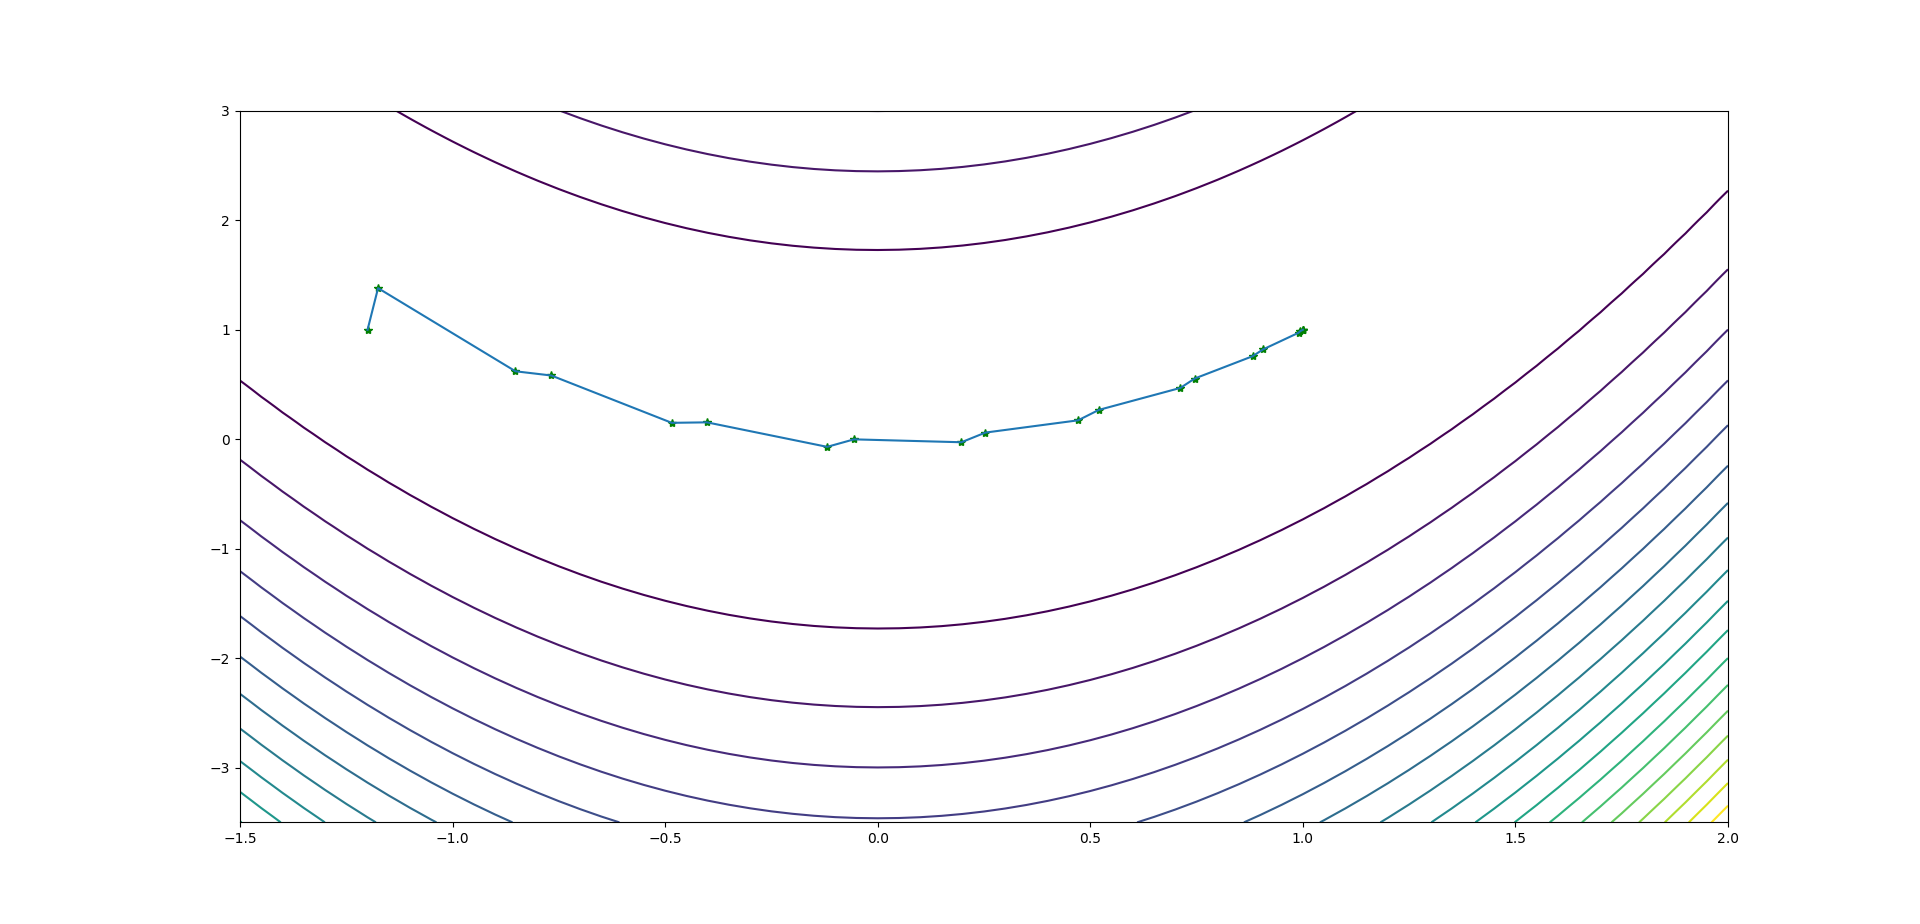
\includegraphics{C:/Users/80693/Desktop/Figure_1-4.png}
%\caption{}
%\end{figure}

第 15 次迭代结果: {[} 0.90650146 0.82113373{]} 步长为: 1 第 16
次迭代结果: {[} 0.98981611 0.97279461{]} 步长为: 1 第 17 次迭代结果: {[}
0.99408025 0.98817735{]} 步长为: 1 第 18 次迭代结果: {[} 0.99997855
0.99992231{]} 步长为: 1 第 19 次迭代结果: {[} 0.99999985 0.9999997 {]}
步长为: 1 第 20 次迭代结果: {[} 1. 1.{]}

可见牛顿法收敛得极快

\begin{Shaded}
\begin{Highlighting}[]
\CommentTok{#-*- coding: UTF-8 -*-}
\CommentTok{"""}
\CommentTok{Newton法}
\CommentTok{Rosenbrock函数}
\CommentTok{函数 f(x)=100*(x(2)-x(1).^2).^2+(1-x(1)).^2}
\CommentTok{梯度 g(x)=(-400*(x(2)-x(1)^2)*x(1)-2*(1-x(1)),200*(x(2)-x(1)^2))^(T)}
\CommentTok{"""}
\NormalTok{rou}\OperatorTok{=}\FloatTok{0.01}
\ImportTok{import}\NormalTok{ numpy }\ImportTok{as}\NormalTok{ np}
\ImportTok{import}\NormalTok{ matplotlib.pyplot }\ImportTok{as}\NormalTok{ plt}
\KeywordTok{def}\NormalTok{ F(x):}
    \ControlFlowTok{return} \DecValTok{100}\OperatorTok{*}\NormalTok{(x[}\DecValTok{1}\NormalTok{]}\OperatorTok{-}\NormalTok{x[}\DecValTok{0}\NormalTok{]}\OperatorTok{**}\DecValTok{2}\NormalTok{)}\OperatorTok{**}\DecValTok{2}\OperatorTok{+}\NormalTok{(}\DecValTok{1}\OperatorTok{-}\NormalTok{x[}\DecValTok{0}\NormalTok{])}\OperatorTok{**}\DecValTok{2}\OperatorTok{;}

\KeywordTok{def}\NormalTok{ jacobian(x):}
    \ControlFlowTok{return}\NormalTok{ np.array([}\OperatorTok{-}\DecValTok{400}\OperatorTok{*}\NormalTok{x[}\DecValTok{0}\NormalTok{]}\OperatorTok{*}\NormalTok{(x[}\DecValTok{1}\NormalTok{]}\OperatorTok{-}\NormalTok{x[}\DecValTok{0}\NormalTok{]}\OperatorTok{**}\DecValTok{2}\NormalTok{)}\OperatorTok{-}\DecValTok{2}\OperatorTok{*}\NormalTok{(}\DecValTok{1}\OperatorTok{-}\NormalTok{x[}\DecValTok{0}\NormalTok{]),}\DecValTok{200}\OperatorTok{*}\NormalTok{(x[}\DecValTok{1}\NormalTok{]}\OperatorTok{-}\NormalTok{x[}\DecValTok{0}\NormalTok{]}\OperatorTok{**}\DecValTok{2}\NormalTok{)])}

\KeywordTok{def}\NormalTok{ hessian(x):}
    \ControlFlowTok{return}\NormalTok{ np.array([[}\OperatorTok{-}\DecValTok{400}\OperatorTok{*}\NormalTok{(x[}\DecValTok{1}\NormalTok{]}\OperatorTok{-}\DecValTok{3}\OperatorTok{*}\NormalTok{x[}\DecValTok{0}\NormalTok{]}\OperatorTok{**}\DecValTok{2}\NormalTok{)}\OperatorTok{+}\DecValTok{2}\NormalTok{,}\OperatorTok{-}\DecValTok{400}\OperatorTok{*}\NormalTok{x[}\DecValTok{0}\NormalTok{]],[}\OperatorTok{-}\DecValTok{400}\OperatorTok{*}\NormalTok{x[}\DecValTok{0}\NormalTok{],}\DecValTok{200}\NormalTok{]])}

\KeywordTok{def}\NormalTok{ phi(a,x,p):}
    \ControlFlowTok{return}\NormalTok{ F(x}\OperatorTok{+}\NormalTok{a}\OperatorTok{*}\NormalTok{p)}


\KeywordTok{def}\NormalTok{ Apha(x,p,g):}
\NormalTok{    a}\OperatorTok{=}\DecValTok{1}
    \ControlFlowTok{while}\NormalTok{(phi(a,x,p)}\OperatorTok{>=}\NormalTok{F(x)}\OperatorTok{+}\NormalTok{rou}\OperatorTok{*}\NormalTok{np.dot(p.transpose(),g)}\OperatorTok{*}\NormalTok{a):}
\NormalTok{        a}\OperatorTok{=}\FloatTok{0.9}\OperatorTok{*}\NormalTok{a}
    \ControlFlowTok{return}\NormalTok{ a}

\NormalTok{X1}\OperatorTok{=}\NormalTok{np.arange(}\OperatorTok{-}\FloatTok{1.5}\NormalTok{,}\DecValTok{2}\OperatorTok{+}\FloatTok{0.05}\NormalTok{,}\FloatTok{0.05}\NormalTok{)}
\NormalTok{X2}\OperatorTok{=}\NormalTok{np.arange(}\OperatorTok{-}\FloatTok{3.5}\NormalTok{,}\DecValTok{3}\OperatorTok{+}\FloatTok{0.05}\NormalTok{,}\FloatTok{0.05}\NormalTok{)}
\NormalTok{[x1,x2]}\OperatorTok{=}\NormalTok{np.meshgrid(X1,X2)}
\NormalTok{f}\OperatorTok{=}\DecValTok{100}\OperatorTok{*}\NormalTok{(x2}\OperatorTok{-}\NormalTok{x1}\OperatorTok{**}\DecValTok{2}\NormalTok{)}\OperatorTok{**}\DecValTok{2}\OperatorTok{+}\NormalTok{(}\DecValTok{1}\OperatorTok{-}\NormalTok{x1)}\OperatorTok{**}\DecValTok{2}\OperatorTok{;} \CommentTok{# 给定的函数}
\NormalTok{plt.contour(x1,x2,f,}\DecValTok{20}\NormalTok{) }\CommentTok{# 画出函数的20条轮廓线}


\KeywordTok{def}\NormalTok{ newton(x0):}

    \BuiltInTok{print}\NormalTok{(}\StringTok{'初始点为:'}\NormalTok{)}
    \BuiltInTok{print}\NormalTok{(x0,}\StringTok{'}\CharTok{\textbackslash{}n}\StringTok{'}\NormalTok{)}
\NormalTok{    W}\OperatorTok{=}\NormalTok{np.zeros((}\DecValTok{2}\NormalTok{,}\DecValTok{10}\OperatorTok{**}\DecValTok{3}\NormalTok{))}
\NormalTok{    i }\OperatorTok{=} \DecValTok{1}
\NormalTok{    imax }\OperatorTok{=} \DecValTok{1000}
\NormalTok{    W[:,}\DecValTok{0}\NormalTok{] }\OperatorTok{=}\NormalTok{ x0}
\NormalTok{    x }\OperatorTok{=}\NormalTok{ x0}
\NormalTok{    delta }\OperatorTok{=} \DecValTok{1}
\NormalTok{    alpha }\OperatorTok{=} \DecValTok{1}

    \ControlFlowTok{while}\NormalTok{ i}\OperatorTok{<}\NormalTok{imax }\KeywordTok{and}\NormalTok{ delta}\OperatorTok{>}\DecValTok{10}\OperatorTok{**}\NormalTok{(}\OperatorTok{-}\DecValTok{10}\NormalTok{):}
\NormalTok{        p }\OperatorTok{=} \OperatorTok{-}\NormalTok{np.dot(np.linalg.inv(hessian(x)),jacobian(x))}
        \CommentTok{#p=-jacobian(x)}
\NormalTok{        x0 }\OperatorTok{=}\NormalTok{ x}
       \CommentTok{# alpha=1.0*np.dot(jacobian(x).transpose(),jacobian(x))/np.dot((np.dot(jacobian(x).transpose(),hessian(x))),jacobian(x))}
\NormalTok{        alpha}\OperatorTok{=}\NormalTok{Apha(x,p,jacobian(x))}
        \BuiltInTok{print}\NormalTok{(}\StringTok{'步长为:'}\NormalTok{)}
        \BuiltInTok{print}\NormalTok{(alpha)}
       \CommentTok{# alpha=1.0}
\NormalTok{        x }\OperatorTok{=}\NormalTok{ x }\OperatorTok{+}\NormalTok{ alpha}\OperatorTok{*}\NormalTok{p}
\NormalTok{        W[:,i] }\OperatorTok{=}\NormalTok{ x}
\NormalTok{        delta }\OperatorTok{=} \BuiltInTok{sum}\NormalTok{((x}\OperatorTok{-}\NormalTok{x0)}\OperatorTok{**}\DecValTok{2}\NormalTok{)}
        \BuiltInTok{print}\NormalTok{(}\StringTok{'第 }\SpecialCharTok\NormalTok{(i))}
        \BuiltInTok{print}\NormalTok{(x)}
\NormalTok{        i}\OperatorTok{=}\NormalTok{i}\OperatorTok{+}\DecValTok{1}
\NormalTok{    W}\OperatorTok{=}\NormalTok{W[:,}\DecValTok{0}\NormalTok{:i]  }\CommentTok{# 记录迭代点}
    \ControlFlowTok{return}\NormalTok{ W}

\NormalTok{x0 }\OperatorTok{=}\NormalTok{ np.array([}\OperatorTok{-}\FloatTok{1.2}\NormalTok{,}\DecValTok{1}\NormalTok{])}
\NormalTok{W}\OperatorTok{=}\NormalTok{newton(x0)}

\NormalTok{plt.plot(W[}\DecValTok{0}\NormalTok{,:],W[}\DecValTok{1}\NormalTok{,:],}\StringTok{'g*'}\NormalTok{,W[}\DecValTok{0}\NormalTok{,:],W[}\DecValTok{1}\NormalTok{,:]) }\CommentTok{# 画出迭代点收敛的轨迹}
\NormalTok{plt.show()}
\end{Highlighting}
\end{Shaded}

\subsection{5.19}\label{header-n133}

\begin{Shaded}
\begin{Highlighting}[]
\NormalTok{N=}\FloatTok{8}\NormalTok{;}
\NormalTok{G=ones(N,N);}
\NormalTok{b=ones(N,}\FloatTok{1}\NormalTok{);}
\NormalTok{x0=zeros(N,}\FloatTok{1}\NormalTok{);}
\NormalTok{for i= }\FloatTok{1}\NormalTok{:N}
\NormalTok{    for j =}\FloatTok{1}\NormalTok{:N}
\NormalTok{         G(i,j) = }\FloatTok{1}\NormalTok{/(i+j-}\FloatTok{1}\NormalTok{);}
\NormalTok{    end}
\NormalTok{end}
\NormalTok{    x = x0;}
\NormalTok{    g = G*x-b;}
\NormalTok{    p = -g;}
\NormalTok{    k = }\FloatTok{0}\NormalTok{;}
\NormalTok{    while }\FloatTok{1}
\NormalTok{        if norm(g, }\FloatTok{2}\NormalTok{)<}\FloatTok{1e-6}
\NormalTok{            break}
\NormalTok{        end}
\NormalTok{        k = k + }\FloatTok{1}\NormalTok{;}
        
\NormalTok{        d=G*p;}
\NormalTok{        a=(g'*g)/(p'*d);}
\NormalTok{        x = x+a*p;}
\NormalTok{        t=g+a*d;}
\NormalTok{       beta=(t'*t)/(g'*g);}
\NormalTok{       g=t;}
\NormalTok{       p=-g+beta*p;}
\NormalTok{    end}
\NormalTok{k}
\NormalTok{x}
\end{Highlighting}
\end{Shaded}

\begin{longtable}[]{@{}llll@{}}
\toprule
n=5 & n=8 & n=12 & n=20\tabularnewline
\midrule
\endhead
k=6 & k=19 & k=35 & k=66\tabularnewline
x & x & x & x\tabularnewline
5.00000002066037 & 5.89856766292802e-11 & -9.60895537135449 &
-10.9749126510893\tabularnewline
-120.000000009110 & -6.97176032007019e-11 & 815.396945500909 &
1050.92924583463\tabularnewline
629.999999984204 & -5.15860286852761e-10 & -16496.5601423969 &
-23956.2795083182\tabularnewline
-1120.00000001358 & 1.12339461172630e-09 & 135510.323445556 &
220425.673599387\tabularnewline
629.999999984357 & 3.17065483551747e-10 & -536481.215700387 &
-965346.669654001\tabularnewline
& -6.55028164772178e-10 & 1025399.39571366 &
1990103.06862559\tabularnewline
& -6.56530674556942e-10 & -642578.292665479 &
-1252700.00760310\tabularnewline
& 4.58964570698870e-10 & -657590.976689034 &
-1343474.30912827\tabularnewline
& & 804243.884701944 & 883233.066644487\tabularnewline
& & 663072.549158718 & 1687963.95092874\tabularnewline
& & -1241279.51532581 & 388212.758339880\tabularnewline
& & 465506.443773192 & -1305525.72041703\tabularnewline
& & & -1710545.71991628\tabularnewline
& & & -528251.066590642\tabularnewline
& & & 1208686.49124660\tabularnewline
& & & 2002890.86386703\tabularnewline
& & & 944594.155587335\tabularnewline
& & & -1434053.34920119\tabularnewline
& & & -2650953.30867554\tabularnewline
& & & 1887855.72260968\tabularnewline
\bottomrule
\end{longtable}

\subsection{5.21}\label{header-n251}

\begin{Shaded}
\begin{Highlighting}[]
\NormalTok{N=}\FloatTok{4}\NormalTok{;}
\NormalTok{G=zeros(N,N);}
\NormalTok{b=[-}\FloatTok{1}\NormalTok{,}\FloatTok{0}\NormalTok{,}\FloatTok{2}\NormalTok{,}\FloatTok{5}\NormalTok{^(}\FloatTok{0.5}\NormalTok{)]}
\NormalTok{x0=zeros(N,}\FloatTok{1}\NormalTok{);}
\NormalTok{for i= }\FloatTok{1}\NormalTok{:N}
\NormalTok{     G(i,i) = }\FloatTok{2}\NormalTok{;}
\NormalTok{end}

\NormalTok{for i= }\FloatTok{1}\NormalTok{:N-}\FloatTok{1}
\NormalTok{    G(i+}\FloatTok{1}\NormalTok{,i)=-}\FloatTok{1}\NormalTok{;}
\NormalTok{    G(i,i+}\FloatTok{1}\NormalTok{)=-}\FloatTok{1}\NormalTok{;}
\NormalTok{end}
\NormalTok{    x = x0;}
\NormalTok{    g = G*x-b;}
\NormalTok{    p = -g;}
\NormalTok{    k = }\FloatTok{0}\NormalTok{;}
\NormalTok{    while }\FloatTok{1}
\NormalTok{        if norm(g, }\FloatTok{2}\NormalTok{)<}\FloatTok{1e-6}
\NormalTok{            break}
\NormalTok{        end}
\NormalTok{        k = k + }\FloatTok{1}\NormalTok{;}
        
\NormalTok{        d=G*p;}
\NormalTok{        a=(g'*g)/(p'*d);}

\NormalTok{        x = x+a*p;}
\NormalTok{        t=g+a*d;}
\NormalTok{       beta=(t'*t)/(g'*g);}
\NormalTok{       g=t;}
\NormalTok{       p=-g+beta*p;}
  
\NormalTok{    end}
\end{Highlighting}
\end{Shaded}

k = 3,程序两次迭代之后就截止

g={[}-2 ,-1 , 1.7639 , 2.4721 {]}

Gg={[}-3 ,-1.7639 , 2.0557 , 3.1803{]}

GGg={[}-4.2361, -2.5836 , 2.6950 , 4.3050{]}

\end{document}
